
\documentclass[8pt]{article}

\usepackage[utf8]{inputenc}

\usepackage{amsmath, bm}
\usepackage{graphicx}
\usepackage{amssymb}
\usepackage{float}
\usepackage{caption}
\usepackage{subcaption}
% set font size to 11pt

% set margin
\usepackage[margin=0.5in]{geometry}

\setlength{\parskip}{\baselineskip}%
\setlength{\parindent}{0pt}%
\setlength{\headsep}{5pt}

\begin{document}

% insert pdf cover page here


\title{Lab report: 3A1 Drag of bluff and streamlined bodies}
\author{lwp26}
\date{November 2023}
\maketitle

\section{Introduction}

The understanding of drag force for various bodies, and flow regimes is crucial to designing efficient transportation in aeronautical and maritime engineering.
In this report, the drag force on a sphere, flat plate and streamlined body is measured and a graph of drag coefficient against Reynolds number is plotted.
The spherical body was tested with and without a turbulence inducing trip wire to investigate the difference.
The flow patterns around the bodies are also visualised using tufts and streamlines.
Each body was placed in the Markham wind tunnel and 12 measurements of drag were taken at $1$mBar intervals of dynamic pressures up to $12$mBar.
A counterweight was used to balance the drag force such that the body remained in the same position.

\section{Theory}

\subsection{Dimensionless Quantities}

The flow is taken to be invicid and in the large section before the contraction of the Markham Tunnel, the velocity is negligible, and so the pressure there is the stagnation pressure $p_0$.
\begin{equation}
    p_0 + 0 = p + \frac{1}{2}\rho_a U^2 \implies U = \sqrt{\frac{2(p_0-p)}{\rho_a}}
    \label{eq1}
\end{equation}
The pressure difference between the large section and working section, $p_0 - p$ is measured by a pressure transducer.
\begin{equation}
    Re = \frac{Ud}{\nu}
    \label{re}
\end{equation}
The drag coefficient is calculated from the drag force, $D$, the frontal area, $S$, and the dynamic pressure.
\begin{equation}
    D = C_d \frac{1}{2} \rho_a U^2 S \implies C_d = \frac{2D}{ \rho_a U^2 S}
    \label{eq3}
\end{equation}
This gives the total drag coefficient from both the body and the wire support structure.
The support structure drag coefficient is given as $C_{d, support} = 0.10$ and so the drag coefficient of the body is calculated by subtracting this from the total drag coefficient.
This value is also assumed to be constant with Reynolds number, but is taken to have an uncertainty which is discussed in the next section.
\begin{equation}
    C_{d, body} = C_{d, total} - C_{d, support}
\end{equation}
The density of air is calculated from measured temperature and atmospheric pressure using the ideal gas law.
\begin{equation}
    \rho_a = \frac{P}{RT}
\end{equation}

\subsection{Calculated Uncertainty}

Sources of uncertainty in calculating Reynolds number in equation \ref{re} is shown below.
\begin{equation}
    u(Re) = u(U) + u(d) + u(\nu)
\end{equation}
The relative uncertainties, $u(d)$ and $u(\nu)$ are negligible compared to $u(U)$ as the diameter was measured to a higher degree of precision and the viscosity change for the uncertainty in measured temperature is also negligible.
\begin{equation}
    u(Re) \approx u(U) = \frac{1}{2}u(p_0-p) + \frac{1}{2}u(\rho_a)
    \label{eq5}
\end{equation}
From considering uncertainty from ideal gas law, .
\begin{equation}
     u(\rho_a) = u(T) + u(P)
\end{equation}

Sources of uncertainty in $C_d$, taking $S=\pi d^2/4$.
\begin{equation}
    u(C_d) = u(D) + u(\rho_a U^2) + u(S) = u(D) + u \left( \frac{1}{2}\rho_a U^2 \right) + 2u(d)
\end{equation}
Substituting equation \ref{eq1} and same reasoning as for equation \ref{eq5} that $u(d)$ is negligible.
\begin{equation}
    u(C_d) \approx u(D) + u(p_0-p)
\end{equation}
However, this is the uncertainty in the total drag coefficient.
The uncertainty in the drag coefficient is found using the uncertainty in the support structure drag coefficient as seen below.
\begin{equation}
    u(C_{d, body}) = \sqrt{u(C_{d, total})^2 + u(C_{d, support})^2}
\end{equation}
The support structure drag coefficient is given as $C_{d, support} = 0.10$, which is assumed to be accurate to the 2 decimal places, and so the absolute uncertainty is $\pm 0.005$.

For completeness, the uncertainty in the corrected drag force is calculated below.
\begin{equation}
    D_{body} = D - D_{support} \implies u(D_{body} ) = \sqrt{u(D)^2 + u(D_{support})^2} \\
\end{equation}
\begin{equation}
    D_{support} = C_{d, support} \frac{1}{2} \rho_a U^2 S \implies u(D_{support}) = u(C_{d, support}) + u \left( \frac{1}{2}\rho_a U^2 \right) + u(S)
\end{equation}
\begin{equation}
    u(D_{support}) \approx u(C_{d, support}) + u(p_0-p)
\end{equation}
From these, the body drag and uncertainty band can be plotted against flow velocity.

\subsection{Measurement Uncertainty}
The measurement of dynamic pressure, $p_0-p$, was done with a calibrated pressure sensor, and so the source of absolute uncertainty is taken at the 2 decimal point precision of the sensor.

The uncertainty in drag reading is harder to quantify, as it was observed to fluctuate at higher speeds.
The setup involved buckets of oil to dampen the fluctuations in the drag force, but this was not completely effective.
Single point measurements were taken at each speed, and so the standard deviation of the drag reading is not known.
Instead the uncertainty in the drag reading is taken to be at the 1 point decimal precision, which is valid at low speeds where the drag reading is stable.
The uncertainty in the correction factor to convert the reading into Newtons is taken to be 0.

The Temperature was measured with a temperature gauge with a precision of $1^oC$ and so the error is $\pm 0.5^oC$. This may seem crude, however, on conversion to Kelvin this gives a small relative uncertainty.

The pressure was measured in inches of mercury, with a very high precision of $0.001$ inches.
Changes in mercury's density for the small temperature changes are also negligible and so the atmospheric pressure has negligible uncertainty.

\section{Results}

\begin{figure}[H]
    \centering
    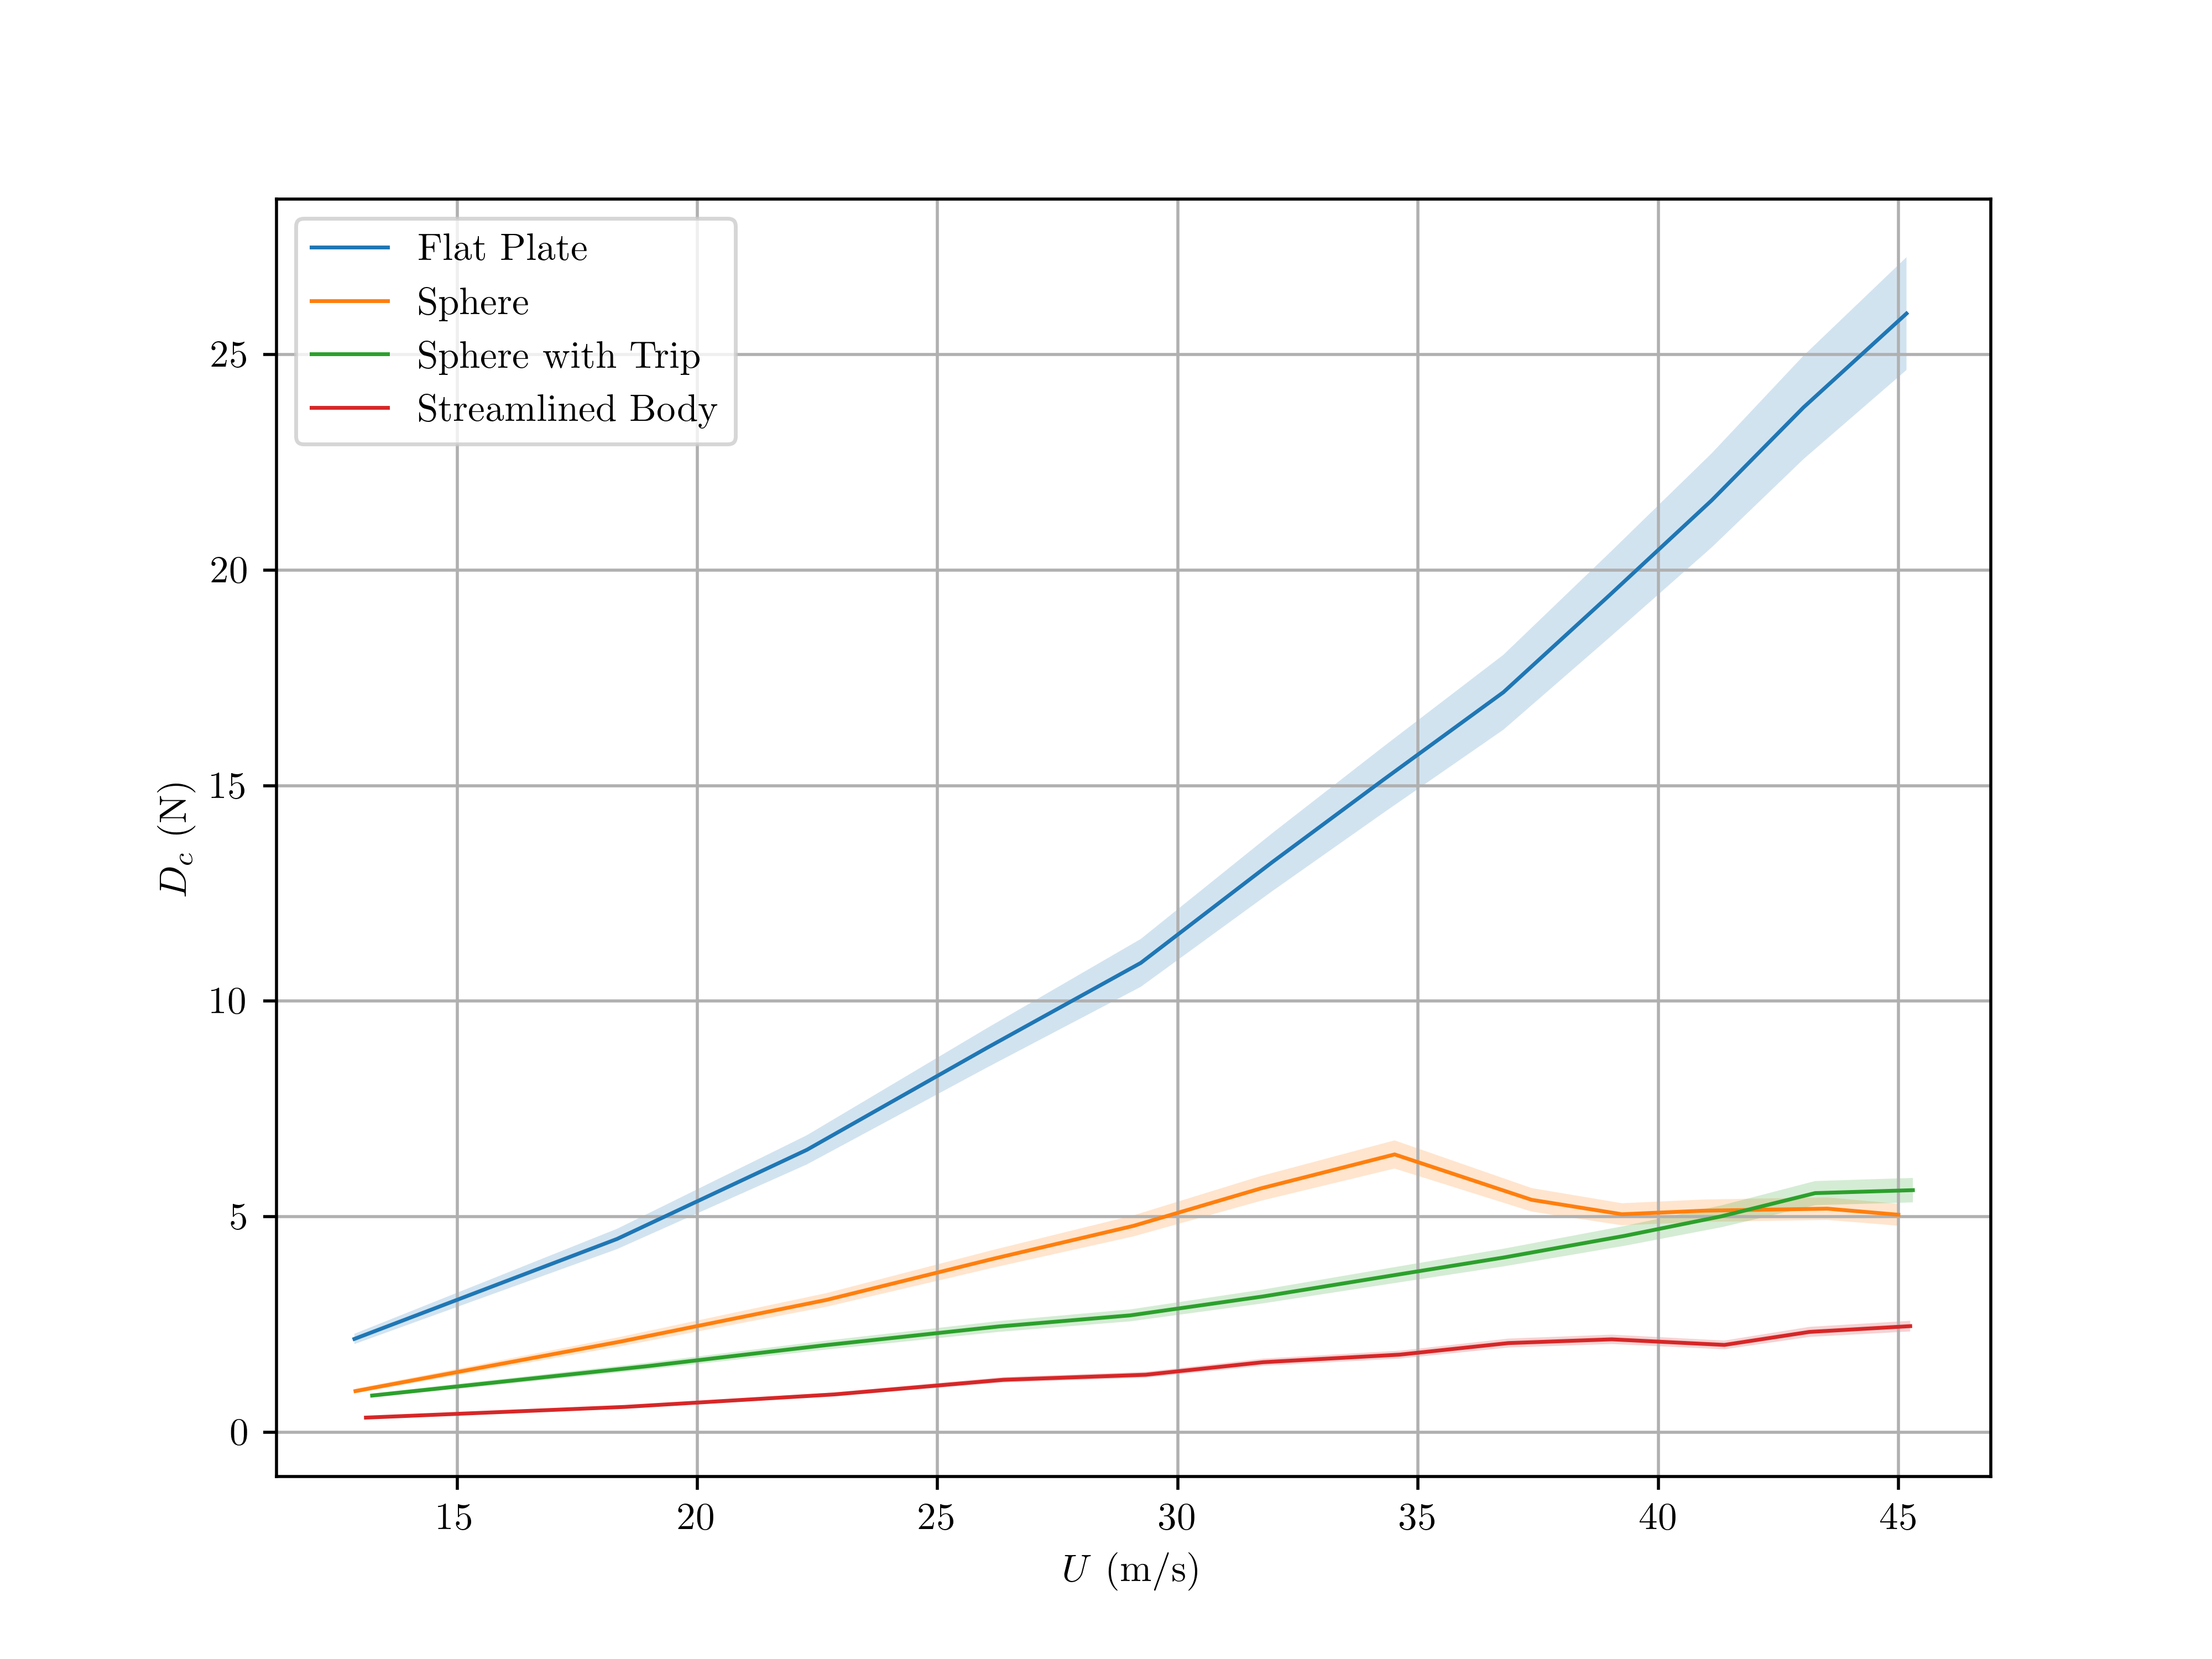
\includegraphics[width=0.75\textwidth]{U_vs_D.png}
    \caption{Graph of corrected drag force, $D_c$ against flow velocity, $U$}
    \label{fig:graph1}
\end{figure}

\begin{figure}[H]
    \centering
    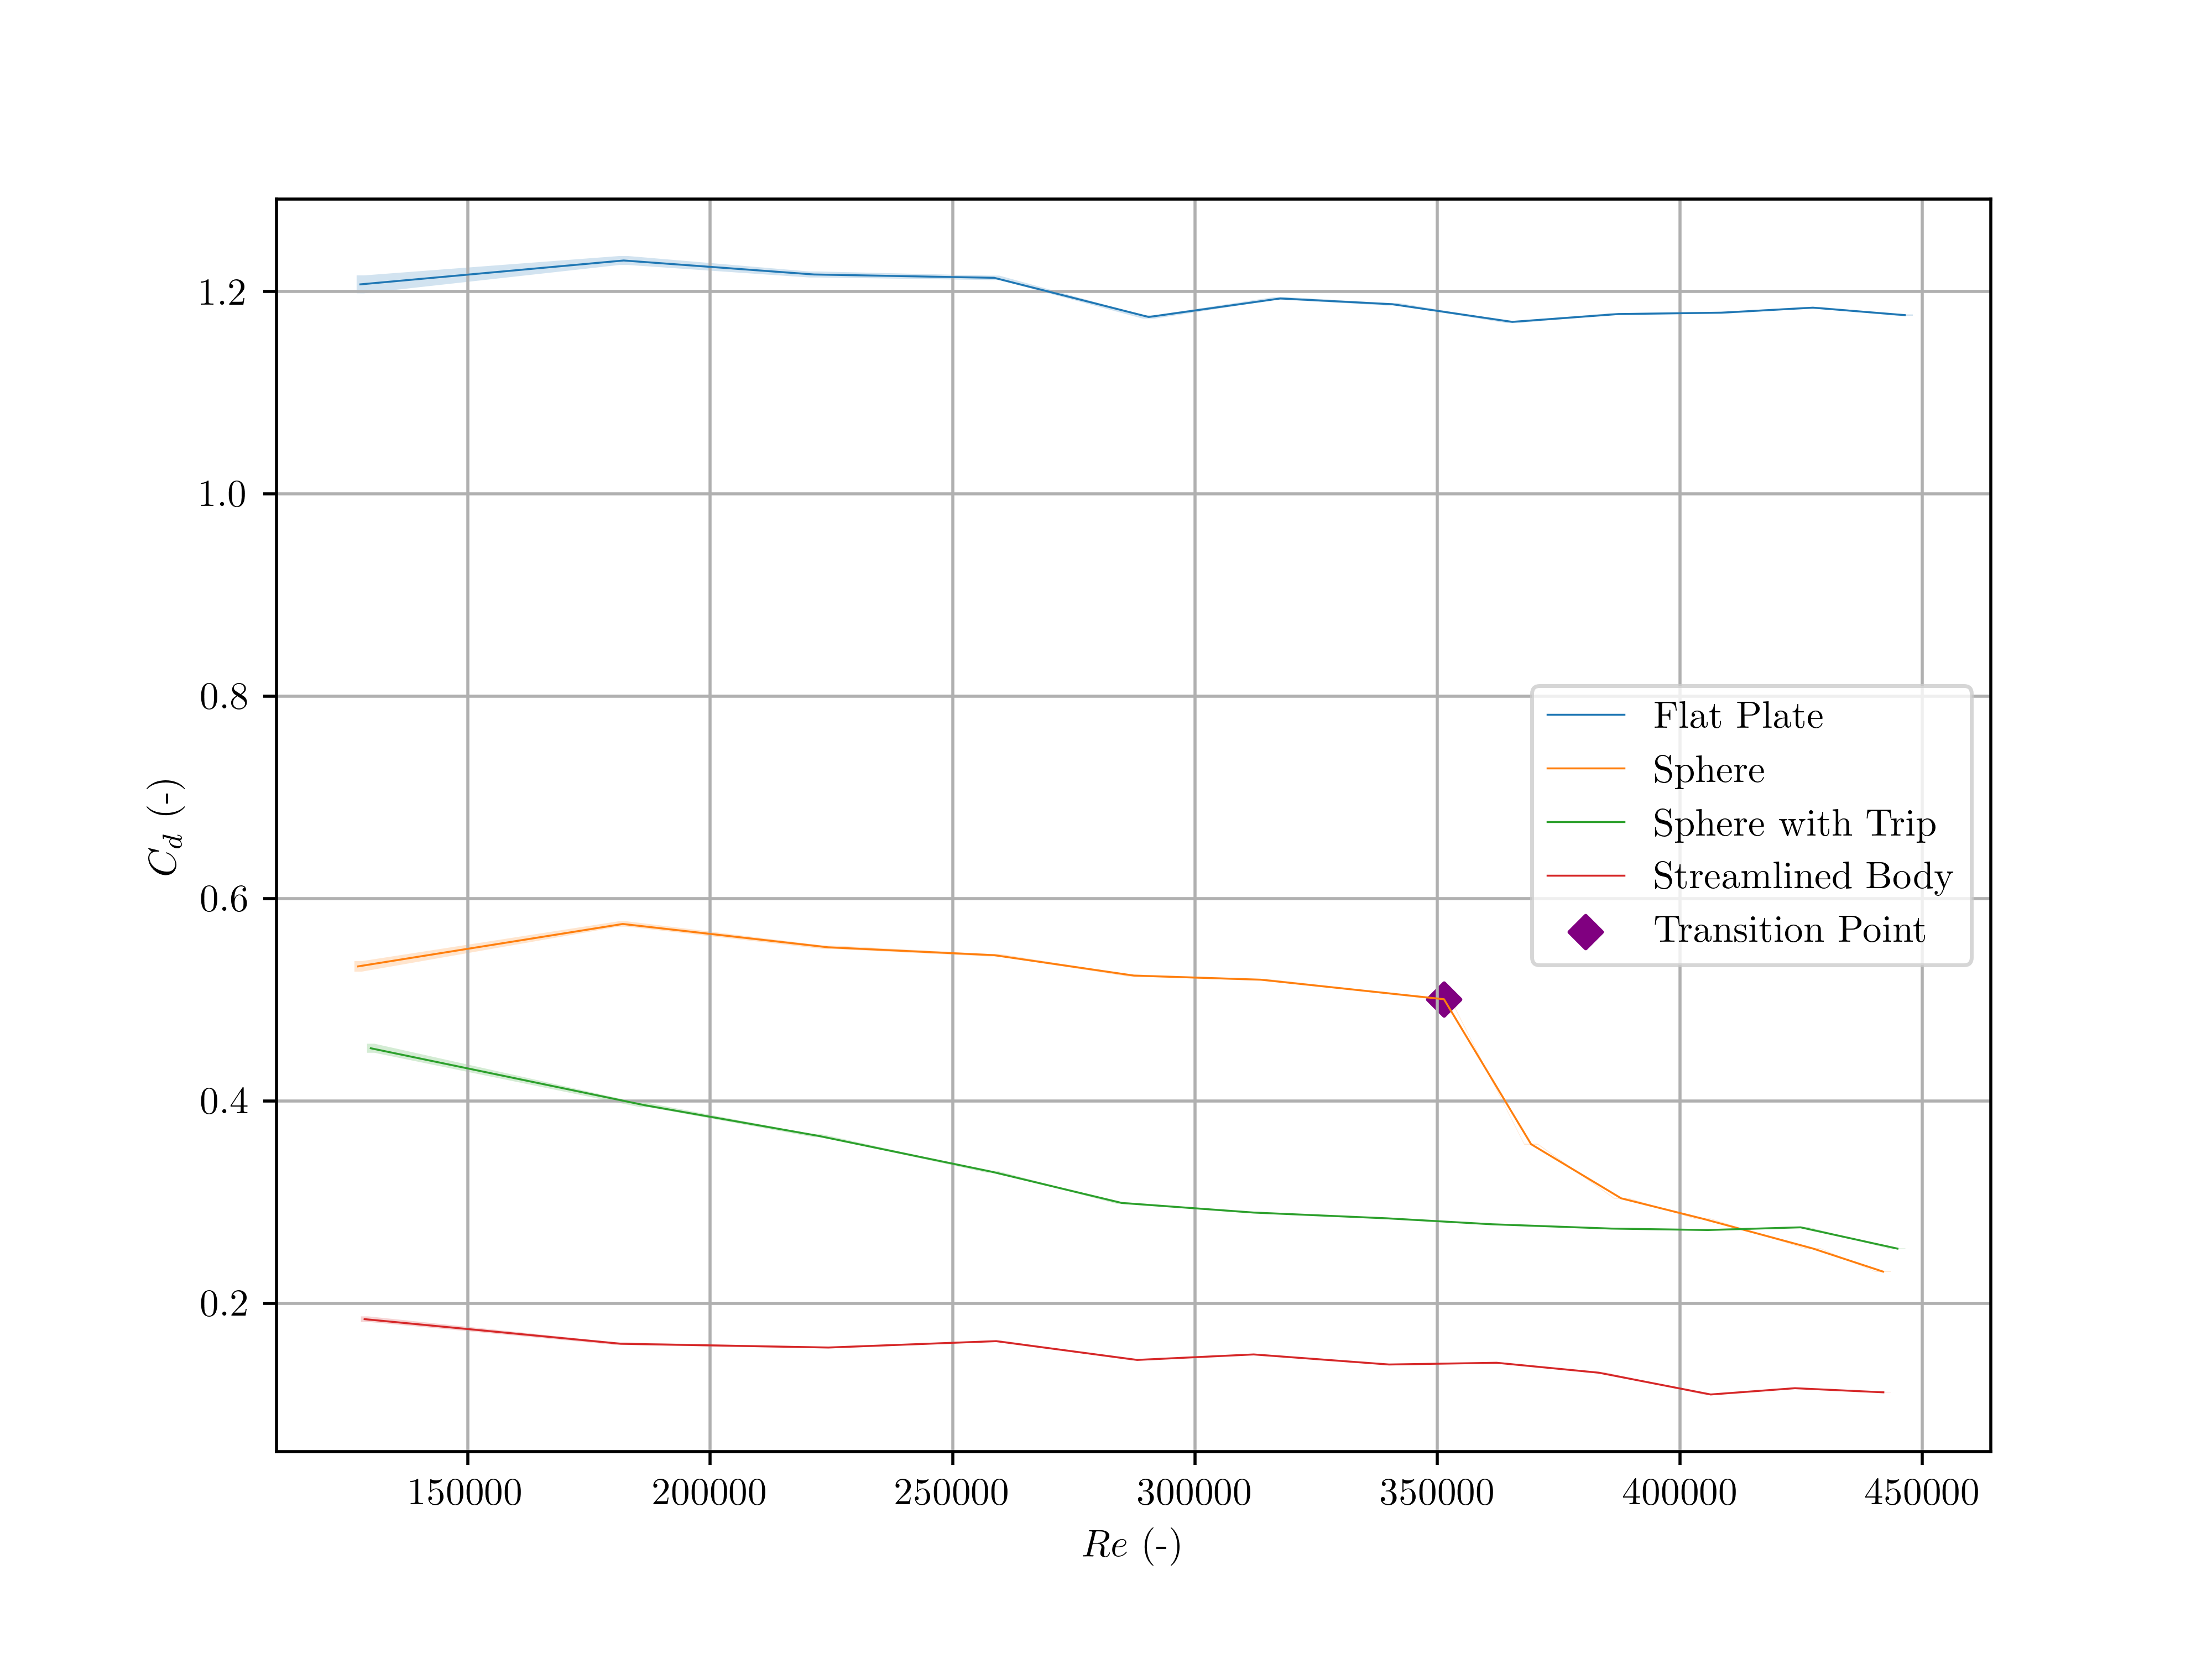
\includegraphics[width=0.75\textwidth]{Re_vs_Cd.png}
    \caption{Graph of drag coefficient against Reynolds number for various bodies}
    \label{fig:figure1}
\end{figure}

\begin{figure}[H]
    \centering
    \begin{subfigure}[t]{0.45\textwidth}
        \centering
        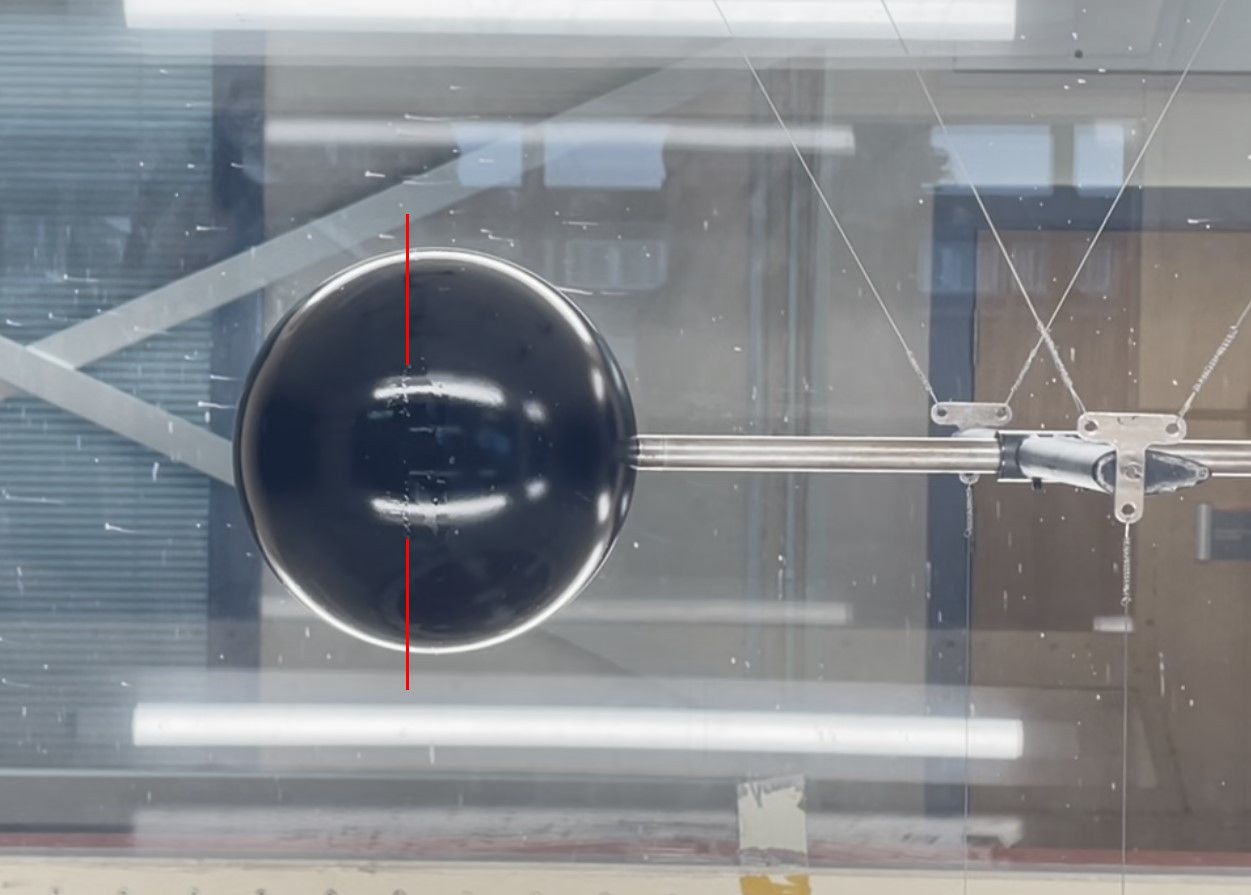
\includegraphics[width=1\textwidth]{Images_Videos/early_seperation_annotated.jpg}
        \caption{Separation before shoulder at low Reynolds number}
        \label{fig:figure2}
    \end{subfigure}
    ~
    \begin{subfigure}[t]{0.48\textwidth}
        \centering
        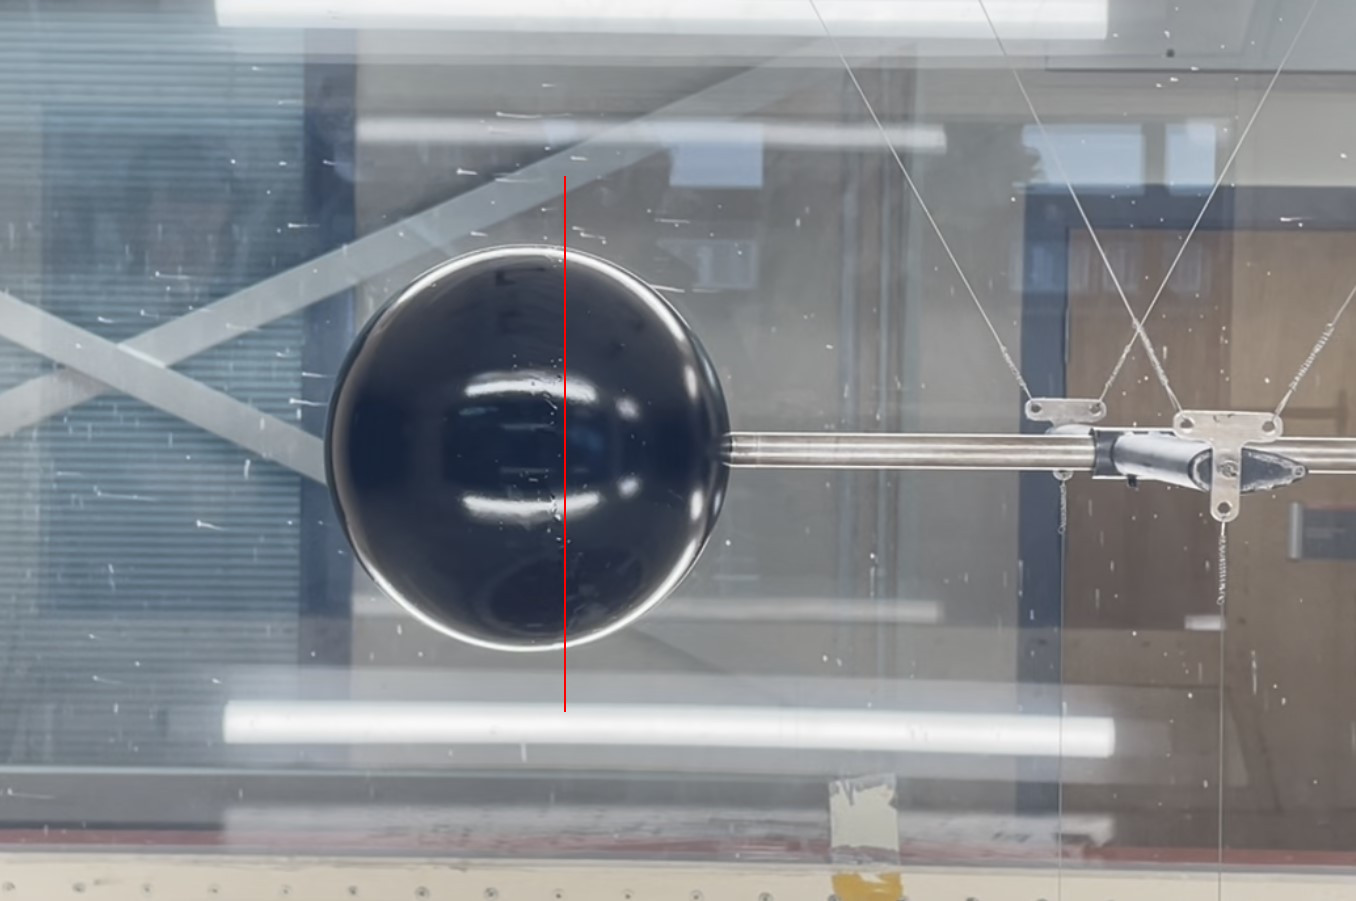
\includegraphics[width=1\textwidth]{Images_Videos/late_seperation_annotated.jpg}
        \caption{Separation after shoulder at high Reynolds number}
        \label{fig:figure3}
    \end{subfigure}
    \caption{Separation points for flow over sphere at low and high Reynolds number indicated by parafin oil}
\end{figure}

\begin{figure}[H]
    \centering
    \begin{subfigure}[t]{0.44\textwidth}
        \centering
        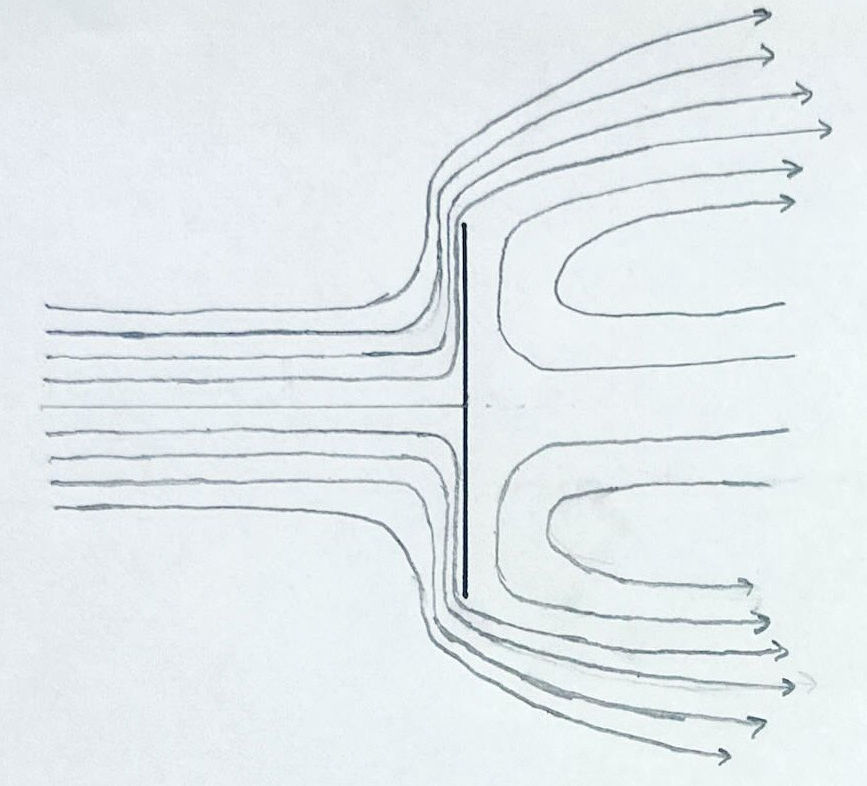
\includegraphics[width=1\textwidth]{Images_Videos/stream_flat_plate_3.jpg}
        \caption{Streamline drawing}
        \label{fig:figure4}
    \end{subfigure}
    ~
    \begin{subfigure}[t]{0.48\textwidth}
        \centering
        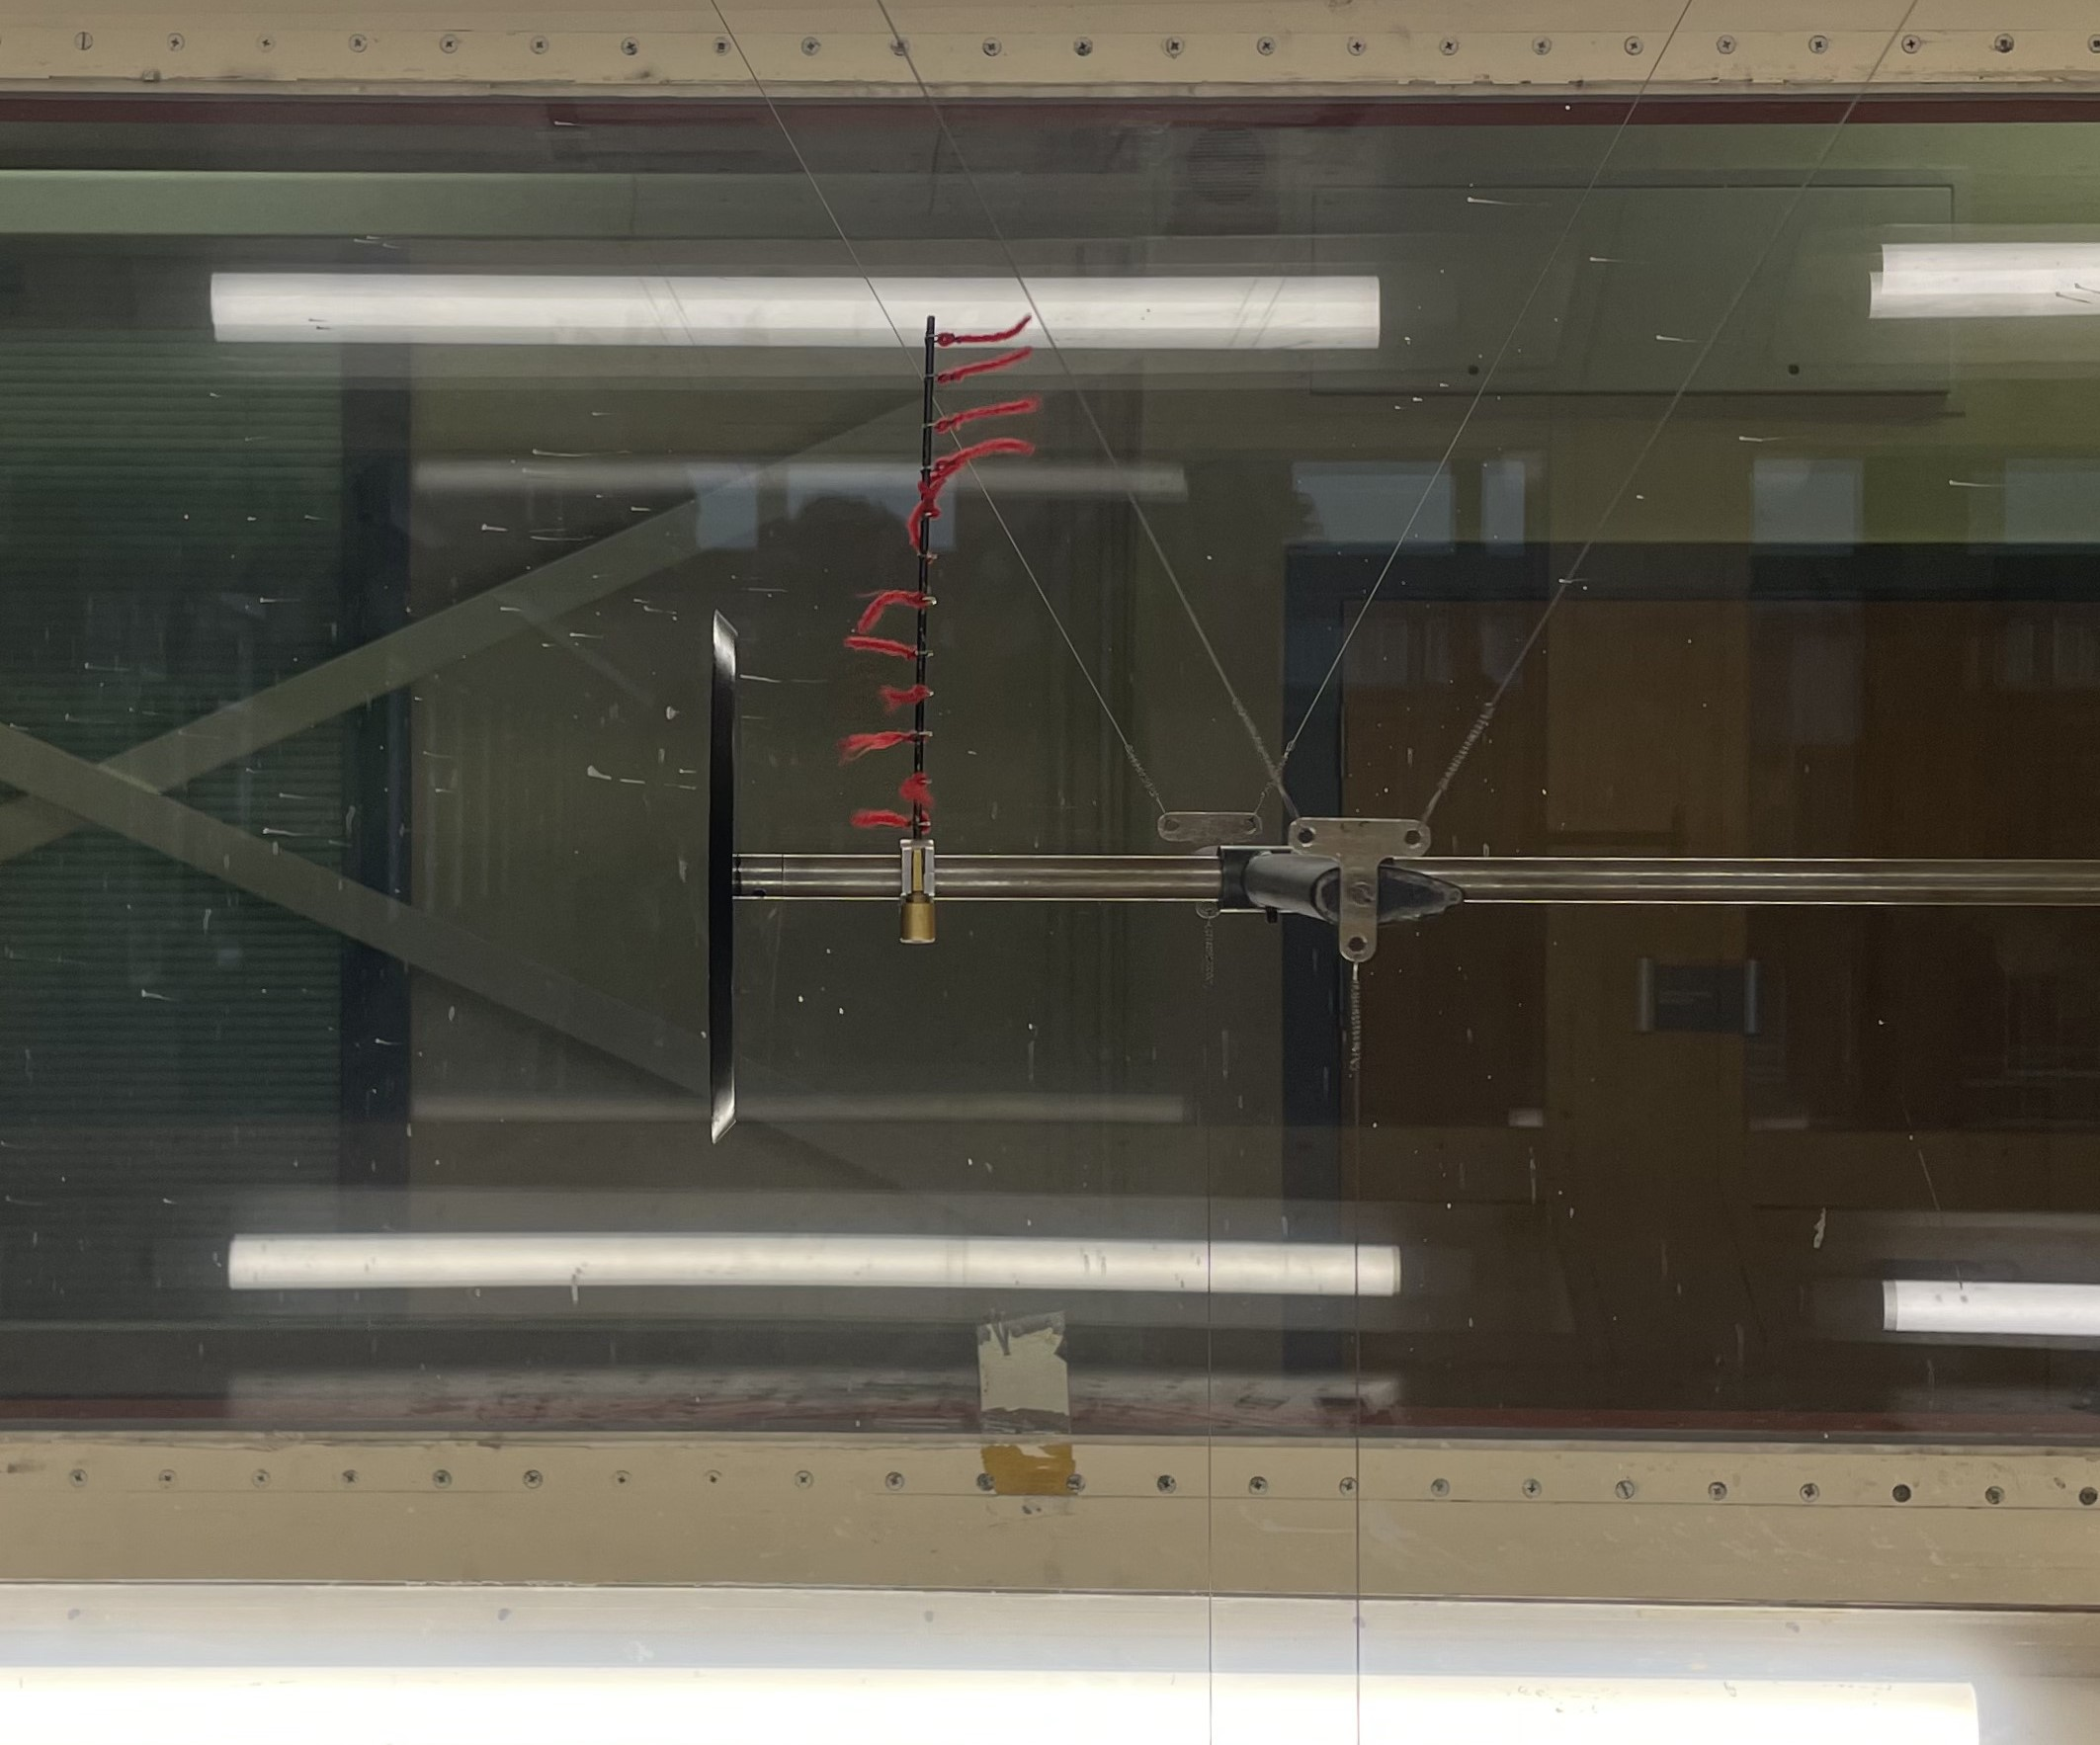
\includegraphics[width=1\textwidth]{Images_Videos/Plate_8milibar_cropped.jpg}
        \caption{Tuft visualisation}
        \label{fig:figure5}
    \end{subfigure}
    \caption{Streamlines and tuft visualisation for flat plate}
\end{figure}

\begin{figure}[H]
    \centering
    \begin{subfigure}[t]{0.48\textwidth}
        \centering
        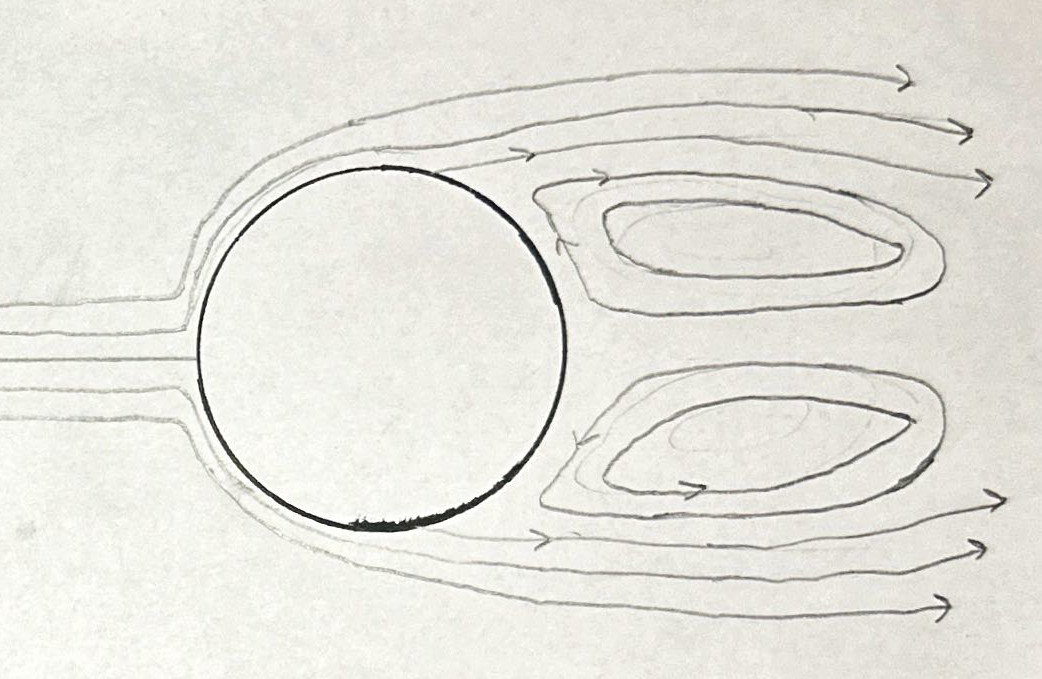
\includegraphics[width=1\textwidth]{Images_Videos/stream_low_Re_sphere_2.jpg}
        \caption{Streamline drawing}
        \label{fig:figure6}
    \end{subfigure}
    ~
    \begin{subfigure}[t]{0.4\textwidth}
        \centering
        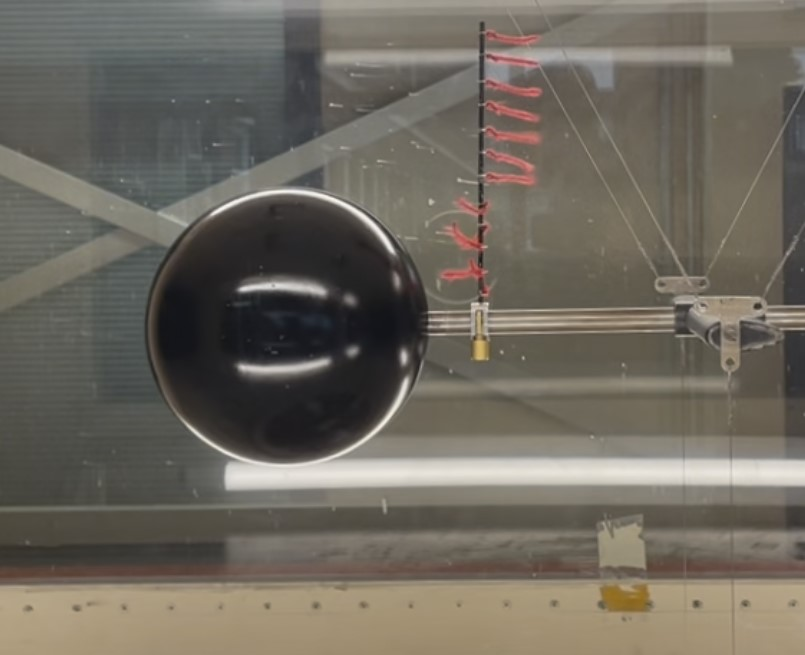
\includegraphics[width=1\textwidth]{Images_Videos/sphere_low_Re.jpg}
        \caption{Tuft visualisation}
        \label{fig:figure7}
    \end{subfigure}
    \caption{Streamlines and tuft visualisation for sphere at low Reynolds number}
\end{figure}

\begin{figure}[H]
    \centering
    \begin{subfigure}[t]{0.48\textwidth}
        \centering
        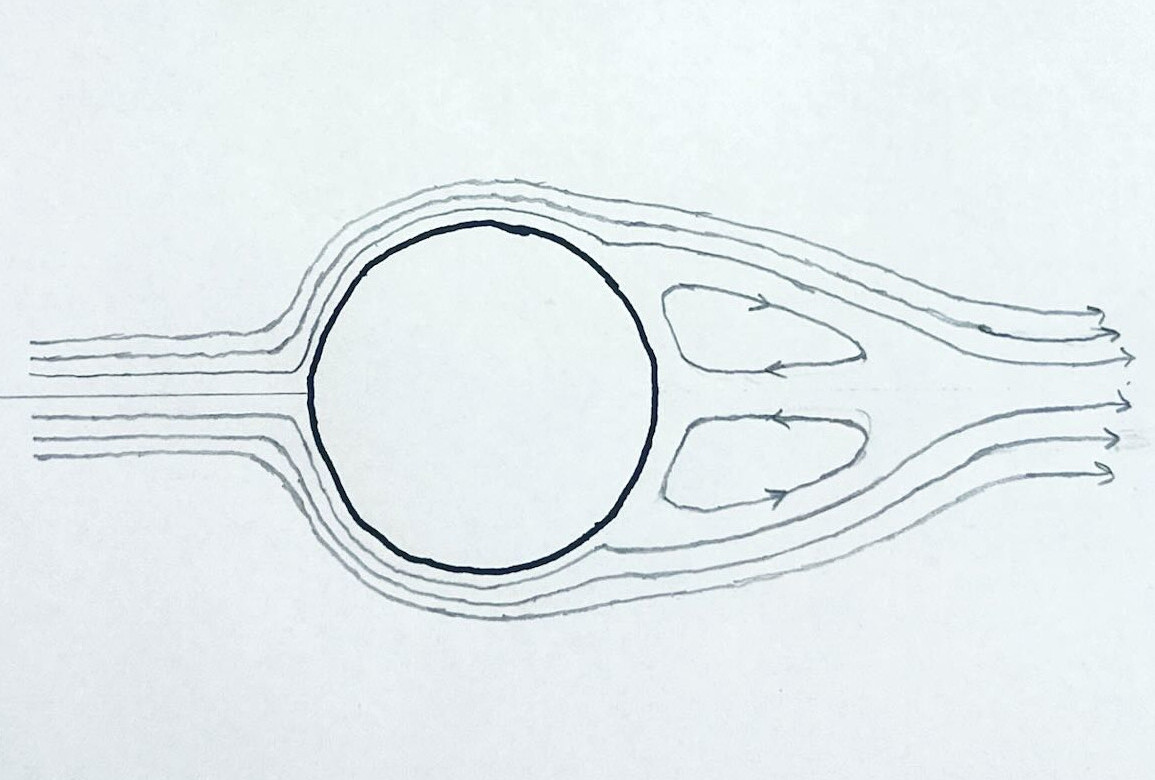
\includegraphics[width=1\textwidth]{Images_Videos/stream_hi_Re_sphere_2.jpg}
        \caption{Streamline drawing}
        \label{fig:figure8}
    \end{subfigure}
    ~
    \begin{subfigure}[t]{0.4\textwidth}
        \centering
        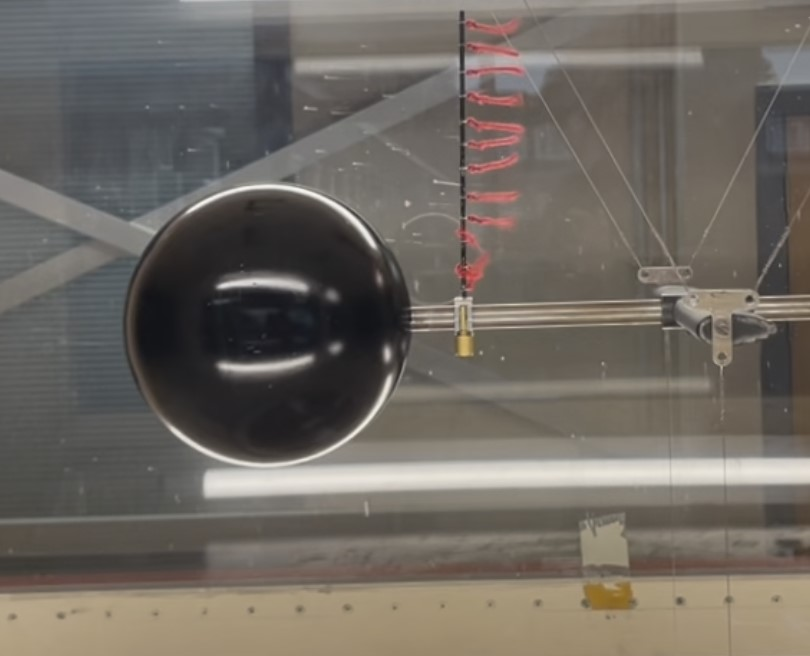
\includegraphics[width=1\textwidth]{Images_Videos/sphere_high_Re.jpg}
        \caption{Tuft visualisation}
        \label{fig:figure9}
    \end{subfigure}
    \caption{Streamlines and tuft visualisation for sphere at high Reynolds number}
\end{figure}

\begin{figure}[H]
    \centering
    \begin{subfigure}[t]{0.48\textwidth}
        \centering
        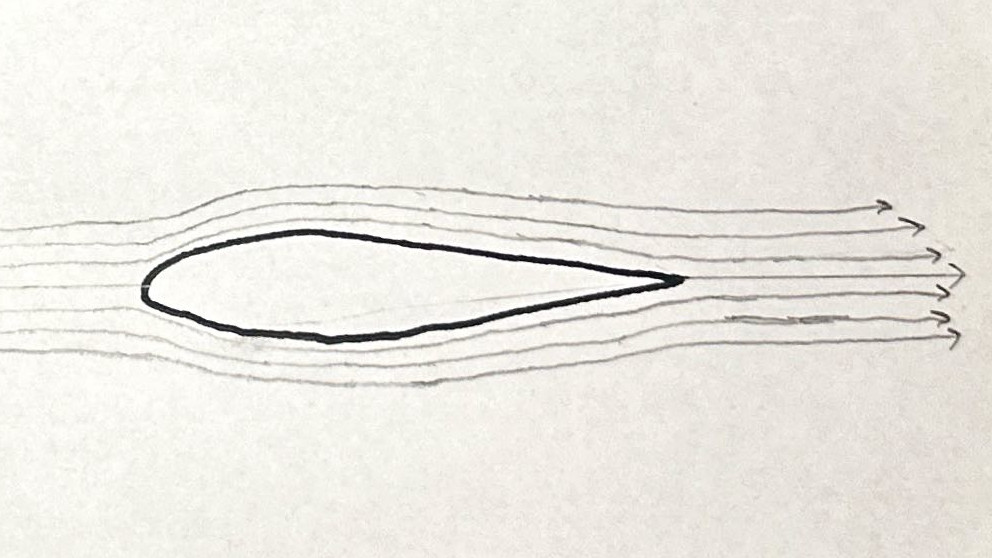
\includegraphics[width=1\textwidth]{Images_Videos/stream_streamlined_2.jpg}
        \caption{Separation before shoulder}
        \label{fig:figure10}
    \end{subfigure}
    ~
    \begin{subfigure}[t]{0.42\textwidth}
        \centering
        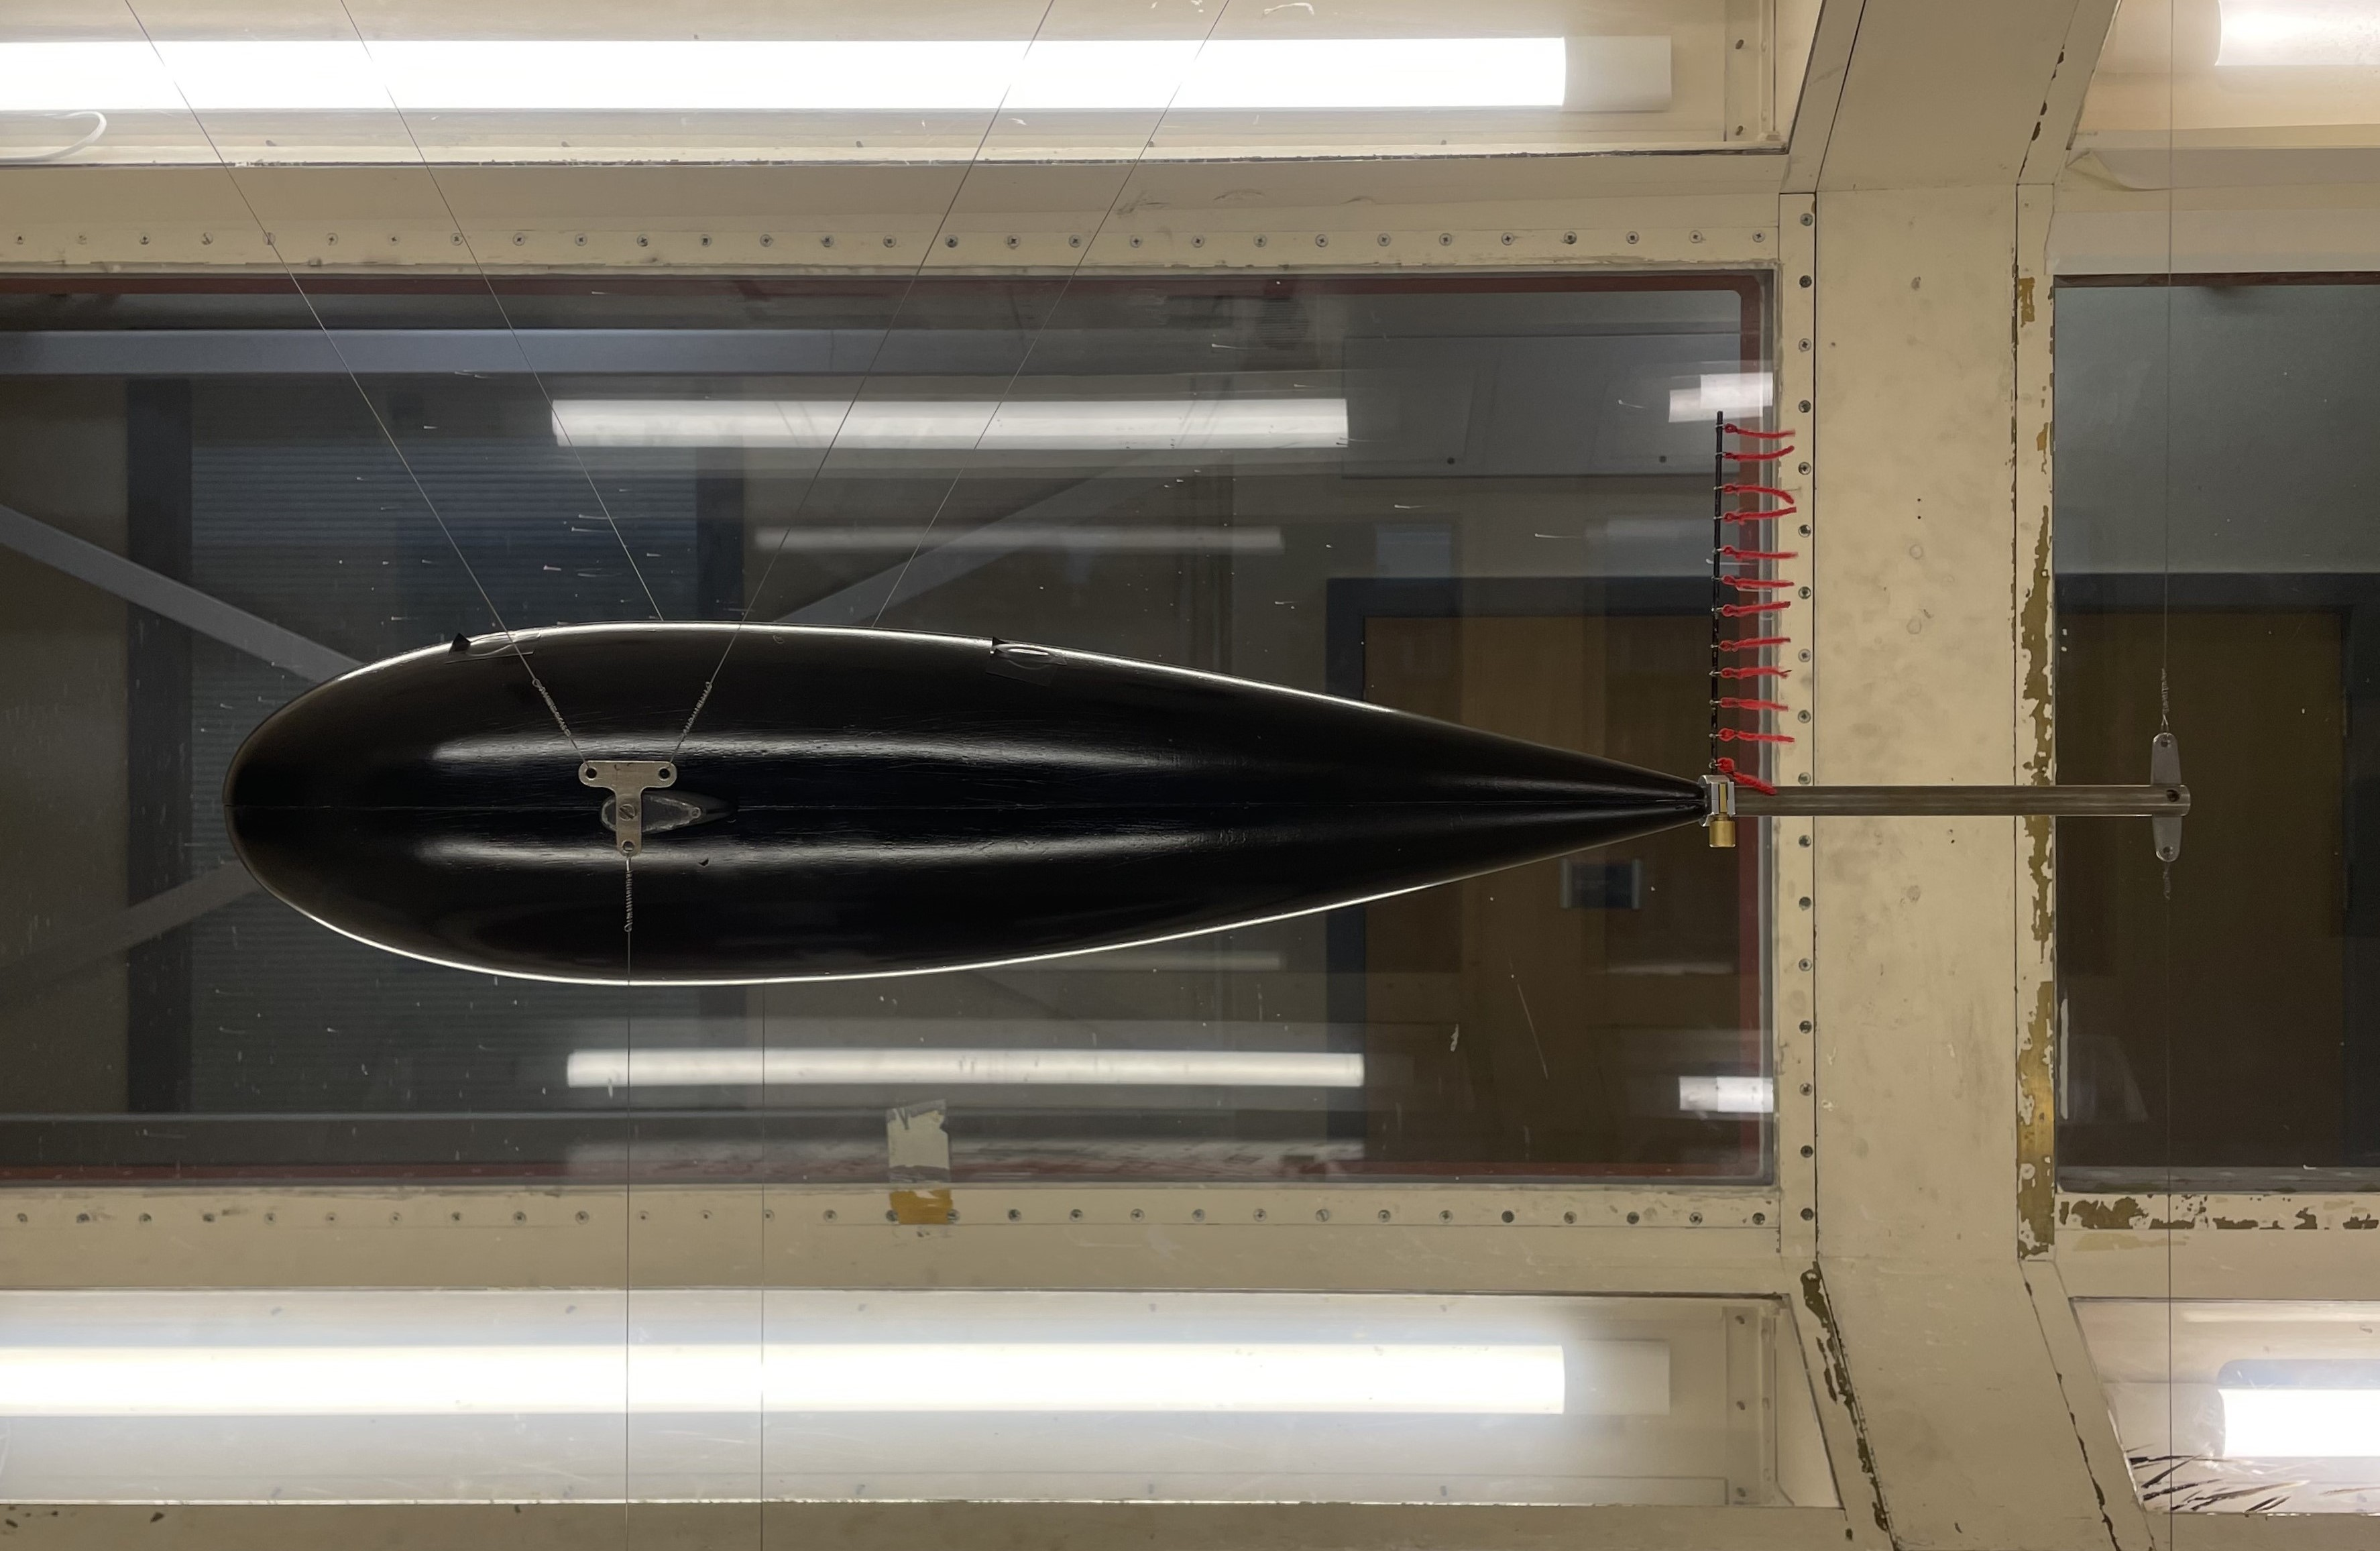
\includegraphics[width=1\textwidth]{Images_Videos/Streamlined_8milibar.JPG}
        \caption{Separation after shoulder at higher Re}
        \label{fig:figure11}
    \end{subfigure}
    \caption{Streamlines and tuft visualisation for streamlined body}
\end{figure}

\section{Discussion}

% 1. Discuss the observations and measurements of the forces and flow fields around the three bodies. Sketch the flow patterns.

From figure \ref{fig:graph1}, the drag force is shown to increase with flow velocity in all cases except the untripped sphere.
However for the untripped sphere, after a critical point, the drag force started to decrease for an increase in flow speed.
Temperature was observed to increase in the tunnel by $3^oC$ over the course of the experiment, which was accounted for in the calculation of air density and tabulated viscosity.
This is caused by the recycled air in the Markham tunnel being heated by the fan compression.

Figure \ref{fig:figure1} shows the plot of drag coefficient, $C_d$ vs Reynolds number, $Re$ for the various bodies. 
For the sphere, the critical Reynolds number where the drag coefficient rapidly decreases is marked on the graph.
This is due to separation occurring behind the maximum circumference shoulder and so the size of the wake is reduced.
The position of separation was confirmed to be behind the shoulder by spraying parafin oil on the sphere and observing where the oil collected on the surface.
Photos of the separation point at low and high Reynolds number are shown in figures \ref{fig:figure2} and \ref{fig:figure3} respectively.

The error is plotted as a transparent band on both figures \ref{fig:graph1} and \ref{fig:figure1}.
The relative uncertainty in both body drag force and body drag coefficient decrease with increasing flow velocity.
This is because both drag and dynamic pressure measurements increase, with constant absolute uncertainty, and so the relative uncertainty in these quantities decreases.
However, the true uncertainty is likely to increase at higher Reynolds number due to the increased fluctuations in the drag reading, not accounted for in the uncertainty analysis.

\newpage




The flow patterns around the bodies were visualised using tufts which are parallel to the streamlines.
These can be seen in figures \ref{fig:figure5}, \ref{fig:figure7} and \ref{fig:figure11} for the flat plate, sphere and streamlined body respectively.
It can be seen that the area of the wake of the flat plate is much larger than the frontal area.
The Flow patterns around the sphere at both low and high Reynolds number were also visualised using tufts in figures \ref{fig:figure7}, and \ref{fig:figure9} respectively.
Figure \ref{fig:figure9} shows an additional tuft below the top of the sphere along a streamline, which shows that the size of the wake is reduced.
This is also shown by separation occurring after the shoulder of the sphere at high Reynolds number, as seen in figure \ref{fig:figure3}.
The tufts behind the streamlined body are shown in figure \ref{fig:figure11}. The streamlines were observed to be effectively parallel and so separation occurs at the end of the body and the area of the wake is negligible.

This reduction in wake significantly reduces the pressure drag.
It can also be seen that the sphere with trip wire has a lower drag coefficient at smaller Reynolds numbers.
This is because the trip wire causes the boundary layer to become turbulent, and so the boundary layer is turbulent for longer, reducing the size of the wake and hence the pressure drag.

% 4. Estimate the errors in the drag coefficients at the lowest speed for all the bodies and mark on your graph. Is the error in the drag coefficient constant? You must include any equations you use to estimate errors in your report.

% This is done in the uncertainty section

% 5. Explain the difference in the Cd versus Reynolds number curves for the different bodies in terms of the flow patterns and the different contributions of form and skin-friction drag.

The various bodies have different contributions to total drag from form and skin friction drag.
The flat plate has the smallest wetted area, and the largest wake. The wetted area is also normal to the drag force, and so the drag force due to the skin friction is negligible.
This suggests that the form drag contributes significantly the total drag force of the flat plate.
The sphere in low Reynolds number flow, separation occurs before the shoulder and so the wake area is slightly larger than the frontal area.
The wetted area is larger than the flat plate, however the form drag is still the significant contributor to the total drag.

Considering the tripped sphere where separation occurs after the shoulder, the wake area is smaller than the frontal area and so the form drag is reduced.
The skin friction drag is increased both due to an increase in wetted area and the now turbulent boundary layer.
Skin friction drag of a turbulent boundary layer is greater than laminar boundary layer due to an increased velocity gradient at the surface as seen in the IB Boundary Layer lab.
Both of these effects contribute to the total drag coefficient.
A rather interesting observation is that as the drag coefficient of the tripped sphere, increases above that of the untripped sphere at higher Reynolds number.
This may be due to the larger turbulent boundary layer of the tripped sphere, as the position of the trip wire is before the shoulder.
However, this is not conclusive due to the fluctuations in drag measurements at higher Reynolds numbers.

The streamlined body has the largest wetted area, and a negligible wake area giving it the smallest drag coefficient of the bodies. 
This suggests that the skin friction drag is the significant contributor to the total drag.

% 6. Explain what is meant by fineness ratio and why there is an optimum for a “streamlined body”.

For a streamlined body, the fineness ratio is defined as the ratio of the length of the body to the diameter of the body.
The form drag is proportional to frontal area and skin friction drag is proportional to wetted area.
The optimum fineness ratio is at the minimum wetted area such that separation occurs at the end of the body.
This minimises the form drag and skin friction drag, giving the minimum total drag coefficient.

\section{Conclusion}

The drag forces of bluff and streamlined bodies were measured and plotted against various flow velocities.
Drag coefficients were calculated and plotted against Reynolds number.
The drag coefficient of the sphere was observed to decrease at a critical Reynolds number which was shown to be due to separation occurring after the shoulder.
Flow at lower Reynolds numbers can be tripped to induce turbulence within the boundary layer, reducing the wake and total drag on a spherical body.
The flow patterns around the bodies were visualised using tufts which were used to draw streamlines and determine wetted and wake areas.
Streamlined bodies have a minimum drag coefficient at a certain fineness ratio, where the wetted area is minimised for no wake.

\end{document}
